\documentclass[b5paper,9pt,twoside,openany]{book}

\usepackage{fontspec,xunicode,xltxtra}
\usepackage{listings}
\usepackage{color}
\usepackage{paralist}
\usepackage{qtree}
\usepackage{dirtree}
\usepackage{pstricks,pst-node}
\usepackage{tabularx}
\usepackage[a5paper]{geometry}
\usepackage[colorlinks=true,linkcolor=blue]{hyperref}


\XeTeXlinebreaklocale ``zh''
\XeTeXlinebreakskip = 0pt plus 1pt minus 0.1pt
\newfontfamily\song{SimSun}
\newfontfamily\hei{SimHei}
%\newfontfamily\kai{KaiTi}
%\newfontfamily\fsong{FangSong}
%\newfontfamily\nsong{NSimSun}
\newfontfamily\mshei{Microsoft YaHei}
\setmainfont{SimSun}

\begin{document} 

\frontmatter
\begin{titlepage}
\raggedleft
{\Large lenxyang@gmail.com\\[1in]}
{\large 基于2.6.11.5\\}
{\Huge\scshape Linux内核分析\\[.2in]}
{\large 以实现的角度\\}
\vfill
{\itshape 2013}
\end{titlepage}

\setcounter{tocdepth}{3}
\tableofcontents
\chapter{前言}
我曾经在一家小公司工作,由于工作需要我们需要制作一个网页分析工具。
这个需求与时下非常流行的机器学习相关,它需要训练集和测试集。
标注数据总是很痛苦且不能简单的找些人来做的工作,为了保证数据的质量,我们必须自己动手。
提高标注的效率就成了关键,当时chrome浏览器已经非常流行,任何用它开发过程前端的同学都应该能够感到它的无比强大。
因此我们的页面标注工具也基于chrome,使用js开发,这个工具很快就搞定了。
但这只是问题的开始,很快我们发现前段标注的数据,以DOM格式存储与后端的DOM格式有极大的不同。
这时候我们才意识到原来DOM与XML不同,它的规范是非常复杂的。
很快一个新的需求被提了出来,我们需要网页的位置信息。


当chromium的核心WebKit被极大简化的时候,性能终于满足的需求,我们可以轻而易举的处理以十亿计的网页了。
它同时产生了一个副产品:我们对WebKit的理解极大的提升。
从那以后,每当看到一个非常好的开源项目的时候,如果我想去学习,我的第一方法总是'简化一边,仅留核心'。


Linux是一个我仰慕已久的开源项目,纵向深入学习却总没时间。
这次终于有时间了,我要尝试用“重构”的方式来学习Linux内核。

于此,我将记录下整个过程,供大家参考,希望也能为更多的人提供一种学习开源项目的方法。
也许他不好,但它的确很适合我。


\mainmatter
\part{初始化阶段}
\chapter{工作环境}

\section{qemu}
\subsection{为什么选用qemu}
比较流行的用于调试内核的虚拟机有很多,Oracle VirtualBox, VMWare, qemu, bochs等等。
前面两款是著名的商业软件,我们暂不考虑。 
作者选用qemu作为虚拟机的原因主要有以下几个
\begin{compactenum}
  \item 内嵌gdbstub调试 这可能是使用它的最大原因了,从虚拟机启动开始就可以直接使用gdb远程调试了,没有比这更然人舒心了。
bochs也包含gdbstub,但需要用户自己编译,如果
  \item 支持多种架构
  \item 速度很快
  \item 安装容易,配置简单,速度快,体积小
\end{compactenum}

\section{bochs}
作为虚拟机bochs的速度真的很慢,但是他内嵌了调试功能,这个对于刚开始接触汇编程序和x86保护模式编程的人来说,真的是不可多得。

直接使用它的内嵌调试器可以查看gdt、idt、 ldt、堆栈等等。这个功能用起来真的非常方便。

举个作者亲身的经历吧,在刚开始学习保护模式编程的时候,作者遇到了一个怪事。
程序倒是很简单,初始化idt, 然后使用ud2触发异常,而后通过汇编程序调用C函数将错误信息打印在屏幕上。
因为涉及到asm调用C程序,作者使用堆栈传递参数,但是push指令却总不起作用。
一怒之下改用寄存器传递参数,发现疑点问题没有。这个问题一定出现在了堆栈上。
于是作者用bochs的dump-stack命令查看堆栈,发现堆栈的地址是16位的,没错它仅仅使用了esp的低16位地址。
回溯代码,作者终于发现原来作者创建的堆栈段是16位的,而我用gdb调试时都是通过观察esp的地址来查看的,所以一直没法查处问题所在。
使用bochs调试器时,它可没有做的先入为主的错误观念,于是很容易发现问题所在。
bochs存在的意义就是帮助我们double-check。
尤其是当你认为是虚拟机bug的时候,多一个虚拟机用来验证总是一件好事。

\subsection{bochs gdbstub}

bochs最大的缺陷就在于没有内嵌gdbstub, 需要用户自己把它编译进去。这也是一个充满各种小坑的路。
作者开始编译的时候使用cygwin配置(configure), 使用VC8编译,编译时成功了,但是一旦gdb成功连接,bochs立马崩溃。
还好后来在cygwin下使用mingw编译成功,如果读者想用,我可以直接把编译成功的binary上传,下载之后应该可以直接使用。

\subsection{cygwin下编译bochs with gdbstub}
前面提到bochs提供的binary是不支持gdbstub的,如果希望编译按照这个说明来实现。它依赖于一些常用工具,我们务必在运行configure脚本之前将它们装好。这些工具的列表在这,相信用过cygwin的朋友们都会安装。
\begin{comptactenum}

\end{compactenum}

\begin{lstlisting}[language=bash]
CC=''/usr/bin/i686-pc-mingw32-gcc''
CXX=''/usr/bin/i686-pc-mingw32-g++''
CFLAGS=''-static-libstdc++ -static-libgcc -O3''
CXXFLAGS=$CFLAGS

export CC
export CXX
export CFLAGS
export CXXFLAGS

./configure  --enable-ne2000 \
    --enable-all-optimizations \
    --enable-cpu-level=6 \
    --enable-x86-64 \
    --enable-pci \
    --enable-clgd54xx \
    --enable-usb \
    --enable-usb-ohci \
    --enable-e1000 \
    --enable-show-ips \
    --enable-gdb-stub \
    --with-win32 --with-rfb --with-nogui
# --enable-sb16
\end{lstlisting}
\section{操作系统}
从开始接触Linux,作者的工作一般都是使用笔记本连接远程开发机的。
这导致一直都不适应linux的桌面环境,如果非用不可的话,作者宁愿安装一个虚拟机然后用putty链接,就好象链接远程机器一样。
在刚开始学习内核编程的时候,作者也一直采用这种方式。
自从cygwin的终端使用putty实现之后,我就毫不犹豫的投入到cygwin的怀抱。
用cygwin就像putty链接虚拟机一样,此外还省去了共享文件,或者远程拷贝文件的麻烦。
cygwin也有它的缺点,xserv连接器了比较麻烦,不过还好我们需要用到的需要x的软件都有windows版。
cygwin的另外一个严重缺点是它之上的编译工具,GNU等生成的代码都是PE文件格式的,不过我们可以通过交叉编译来解决这个问题。
\section{开发工具}

上面提过cygwin下集成的gcc,mingw等开发工具生成的程序都是可以直接在windows下运行的。
因为它产生的是PE文件,一种windows采用的文件格式。
但是我们的内核可是linux的,为此我们需要生成ELF格式的可支持文件,没办法我们必须生成一组交叉编译工具。

如果读者使用Linux作为桌面开发环境有一点也需要注意,本书的内容全部基于i386开发,即:32位操作系统。
但目前流行的Linux已经全部是64位了,所以大家在编译的时候也需要指定arch位i386啊。

\section{第一个程序}

万事俱备,我们用一个程序来启动机器吧。
\begin{lstlisting}
	.code16
	.text
_start:	
	movw	%cs, %ax
	movw	%ax, %ds

	movl	$0x7FF0, %esp
	xor	%ebp, %ebp
1:
        jmp     1b;

__puts:
	pusha
	xor	%bh, %bh
.Lputs1:
	lodsb
	test	%al, %al
	jz	.done
	movb	$0x0e, %ah
	int	$0x10
	jmp	.Lputs1
.done:	
	popa
	ret
msg:
	.asciz	"Hello, Kernel...\r\n"
.org 510
	.word	0xAA55
\end{lstlisting}
\subsection{编译运行}

\chapter{系统加载}

在上一章我们的程序已经取得了机器的控制权,但是他只能做些无聊的事情:打印些东西而后空转。本章它将开始并完成的它的历史使命“加载内核并运行“,不过这个内核会它一样无聊,还是打印些东西然后空转。不过这确实巨大的进步,因为我们的程序已经从汇编变成了带有C的汇编,而且被加载的程序不再受到512字节的限制,它有着无限的可能性。
\section{PC启动程序}
\subsection{读磁盘}
\subsection{ELF文件格式}
\subsection{准备一个ELF格式的内核}
\subsection{开启20位寻址}
系统开机以后,CPU运行于实模式下且仅仅支持16位寻址。这就意味着我们最多可以使用64K的内存。对于bootsect.S的内部处理这个空间应该够用了,但如果想要加载vmlinux这个巨大的程序可以远远不够的。为此我们需要将寻址空间提高的20位,即1M。这也意味着我们的操作系统最多也就只能有1M的大小,这对于一个没有什么驱动程序的操作系统来说足够用了。
\subsection{加载}
为了能够将内核加载到高于64K的内存,我们付出了很多努力,与对任何一个超过64K的内存,我们必将将它分成两个部分存储。实际上,实模式也是可以访问4G物理内存的。接下来我们做个实验看看如何做到这一点,不然的话,我们怎么能像Linux那样将内核加载到1M内存之上呢,而且vmlinux的可是很大的一个文件,1M的寻址空间一定是不够的。
\subsection{打开4G内存访问}
实际上,每一个段寄存器都有可以分两个部分,可见部分(visible part)和隐藏部分(hidden part)。其中隐藏部分有时候叫做descriptor cache或者shadow register。后面保护模式章节会提到,保护模式下段寄存器保存的是selector,读者可以简单的理解成数组的下标,在每次使用selector的时候,CPU都需要查表。这明显会影响效率,CPU提供了一种机制在查表的时候顺便将GDT的值存放在段寄存器的不可见部分,因此它又叫做descriptor cache,因此段寄存器部分的格式就是descriptor的格式,它的具体格式如下图所示:
\begin{pspicture}
\end{pspicture}
这里仅仅介绍与内存相关的部分就好,其它的细节还会在“保护模式“当中详细介绍。

通过修改在修改段寄存器具体内容的时候,它的隐含部分也会更改。利用这种机制可以实现4G的

修改CS隐含部分的值需要使用模式切换,但CPU进入到保护模式的时候,段寄存器的隐含部分自动改变它的状态,但从保护模式且会real-mode,段寄存器的属性则不会改变,我们就利用这个技巧使boot程序能够访问4G内存。
还是通过代码来说明如何打开real-mode下的4G访问
\begin{lstlisting}
        .code16
        .text

.equ    __CODE32_CS,    0x8
.equ    __DATA32_DS,    0x10
.equ    __CODE16_CS,    0x0

        .global _start
_start:
        mov     %cs, %ax
        mov     %ax, %ds
        mov     %ax, %ss
        mov     $0x7c00, %sp

        lgdt    gdtptr

        /* 打开保护模式 */
        mov     %cr0, %eax
        or      $0x1, %eax
        mov     %eax, %cr0

        /* 进入保护模式 */
        .byte   0x66, 0xea
        .long   pm
        .word   0x8

        .code32
pm:
        mov     $__DATA32_DS, %eax
        mov     %eax, %ds
        mov     %eax, %fs
        mov     %eax, %gs

        /* 关闭保护模式 */
        mov     %cr0, %eax
        and     $0xFFFFFFFE, %eax
        mov     %eax, %cr0

        .byte   0x66, 0xea
        .long   real
        .word   __CODE16_CS

        .code16
real:
        mov     $0x7c00, %sp

        mov     $1234, %eax
        mov     $0x100000, %edx
        mov     %eax, (%edx)

        .loop:
        jmp     .loop
gdt:
        .quad   0x0000000000000000 /* NULL selector */
        .quad   0x00cf9a000000ffff /* base=0, limit=0xffff, DPL=0 */
        .quad   0x00cf92000000ffff /* base=0, limit=0xffff, DPL=0 */
gdtptr:
        .word   gdtptr - gdt
        .long   gdt
        .word   0
.org    510
        .word   0xAA55
\end{lstlisting}

\subsubsection{验证}
如何验证呢? 我们不用程序的方式来验证,该有调试器的方式验证,这样做可以避免由于我们理解不到位造成错误。试想如果对内存的理解方式有问题,按照同样的方式写入熟读到内存然后再按照同样的方式读出内存,那结果是一样的,但我们真的不数据写入到了我们希望的那段内存了吗?如果发生了“×××”怎么办,我们根本不知道。比较好的方法就是使用两种不同方式,比如使用自己的程序写入内存,而后用内置调试器来访问物理内存验证数据,这种方法可以确保万无一失。
接下来将使用bochs内置调试器来验证,这样做的原因很简单,gdb远程调试的方式无法获得CPU的状态,某些状态gdb根本就不支持,比如gdt的内容、sreg的隐含部分都无法通过gdb来查看。bochs专门针对x86平台开发,有强大查看CPU内核状态的工具。
\begin{lstlisting}[language=bash]
<bochs:> break *0x7c00
<bochs:> c
<bochs:> n...
<bochs:27> sreg
es:0x0000, dh=0x00009300, dl=0x0000ffff, valid=1
        Data segment, base=0x00000000, limit=0x0000ffff, Read/Write, Accessed
cs:0x0000, dh=0x00cf9300, dl=0x0000ffff, valid=1
        Data segment, base=0x00000000, limit=0xffffffff, Read/Write, Accessed
ss:0x0000, dh=0x00009300, dl=0x0000ffff, valid=7
        Data segment, base=0x00000000, limit=0x0000ffff, Read/Write, Accessed
ds:0x0010, dh=0x00cf9300, dl=0x0000ffff, valid=7
        Data segment, base=0x00000000, limit=0xffffffff, Read/Write, Accessed
fs:0x0010, dh=0x00cf9300, dl=0x0000ffff, valid=1
        Data segment, base=0x00000000, limit=0xffffffff, Read/Write, Accessed
gs:0x0010, dh=0x00cf9300, dl=0x0000ffff, valid=1
        Data segment, base=0x00000000, limit=0xffffffff, Read/Write, Accessed
ldtr:0x0000, dh=0x00008200, dl=0x0000ffff, valid=1
tr:0x0000, dh=0x00008b00, dl=0x0000ffff, valid=1
gdtr:base=0x0000000000007c51, limit=0x18
idtr:base=0x0000000000000000, limit=0x3ff
\end{lstlisting}

再向后过 mov \%eax, (\%edx)之后,验证内存是否已经写入
\begin{lstlisting}[language=bash]
bochs:31> x 0x100000
[bochs]:
0x0000000000100000 <bogus+       0>:    0x000004d2
\end{lstlisting}
4d2为1234的16进制表示,我们确实成功了。

\subsection{真实世界的vmlinux}
为了给大家呈现一个简单的世界,作者自己实现了一个内核加载程序。这个程序加载简化的内核足够用了,但对于真实的linux内核,他是绝对不够用的。原因很简单,vmlinux如果包含调试信息的话有200M那么大,在实模式下是绝对无法加载的。真实世界的linux通常是由GRUB加载,当然还有其他的加载器。GRUB基本上已经是一个小型的操作系统了。它支持与Linux相同的驱动程序框架,并且包含了很多驱动程序,比如ext2,msdos等文件系统的驱动。当然为了统一支持他们,还需要VFS。此外还携带一个shell。当然它不支持操作系统的高级特性,比如复杂的内存管理,多进程的切换和调度,它都没有。但它一定是运行在保护模式下的,在完成加载之后回到实模式,而后将控制权交给目标操作系统。在我们的简化操作系统基本成型以后,我们会尝试使用GRUB2来加载我们的系统。
\section{调试技巧}

程序已经可以运行了,接下来我们熟悉一些调试技巧,这对我们将来开发非常有用。俗话说程序是三分编七分调。程雪写完也就是完成了三成的工作而已,真正复杂的是调试呕。

只要是程序就一定有bug。尤其是按照前面我们所鼓励的方式:将代码抄进文件编译运行。如果有时间作者强烈推荐这种方式,它能够增强你对系统的理解。但这种方式一定会让你的程序存在bug,之前已经介绍了qemu自身就带有gdbstub。让我们一起感受他的强大吧。
\subsection{gdb远程调试}
\begin{lstlisting}[language=bash]
 symbol-file out/arch/i386/boot/bootsect.gdb
 set architecture i8080
 target remote :1234
 hbreak *0x7c00
\end{lstlisting}

\subsection{symbol-file}
前面介绍过,启动程序必须控制在512字节,而且它必须是binary格式的。所谓binary格式就是CPU可以从第一个字节开始运行的程序。因此调试信息是不可能存在与binary之上的。不过大家不用担心,因为我们还生成了一个ELF文件,这个文件包含完整的调试信息。
调试信息大概是什么样子呢?objdump可以帮助大家来理解调试信息看起来是什么样子?正如刚才提到,make之后生成了两个文件bootsect.gdb和bootsect.bin,bootsect.gdb包含完整信息,而bootsect.bin仅仅包含程序。我们用objdump来查看反汇编一下bootsect.gdb的内容,大家可以看到
\begin{lstlisting}[language=bash]
$ objdump.exe  -dl arch/i386/boot/bootsect.gdb

arch/i386/boot/bootsect.gdb:     file format elf32-i386


Disassembly of section .text:

00007c00 <_start>:
arch/i386/boot/bootsect.S:17
    7c00:       8c c8                   mov    %cs,%eax
arch/i386/boot/bootsect.S:18
    7c02:       8e d8                   mov    %eax,%ds
arch/i386/boot/bootsect.S:19
    7c04:       8e c0                   mov    %eax,%es
arch/i386/boot/bootsect.S:20
    7c06:       8e e0                   mov    %eax,%fs
arch/i386/boot/bootsect.S:21
    7c08:       8e e8                   mov    %eax,%gs
arch/i386/boot/bootsect.S:23
    7c0a:       66 bc f0 7f             mov    $0x7ff0,%sp
    7c0e:       00 00                   add    %al,(%eax)
arch/i386/boot/bootsect.S:24
    7c10:       66 31 ed                xor    %bp,%bp
arch/i386/boot/bootsect.S:29
    7c13:       fa                      cli
arch/i386/boot/bootsect.S:30
\end{lstlisting}
这就是调试信息,它将源代码文件与地址对应起来。在我们进行反汇编的时候,它用显示源代码而非反汇编代码。那么反汇编代码看起来如何呢?

\begin{lstlisting}[language=bash]
$ objdump.exe  -d arch/i386/boot/bootsect.gdb

arch/i386/boot/bootsect.gdb:     file format elf32-i386


Disassembly of section .text:

00007c00 <_start>:
    7c00:       8c c8                   mov    %cs,%eax
    7c02:       8e d8                   mov    %eax,%ds
    7c04:       8e c0                   mov    %eax,%es
    7c06:       8e e0                   mov    %eax,%fs
    7c08:       8e e8                   mov    %eax,%gs
    7c0a:       66 bc f0 7f             mov    $0x7ff0,%sp
    7c0e:       00 00                   add    %al,(%eax)
    7c10:       66 31 ed                xor    %bp,%bp
    7c13:       fa                      cli
    7c14:       e4 92                   in     $0x92,%al
    7c16:       0c 02                   or     $0x2,%al
    7c18:       e6 92                   out    %al,$0x92
    7c1a:       fb                      sti
    7c1b:       e8 82 01 be ba          call   babe7da2 <ELFDATA_ADDR+0xbabc7da2>
    7c20:       7d e8                   jge    7c0a <_start+0xa>
    7c22:       6c                      insb   (%dx),%es:(%edi)
    7c23:       01 b8 00 20 8e c0       add    %edi,-0x3f71e000(%eax)
    7c29:       bf 00 00 b8 01          mov    $0x1b80000,%edi
    7c2e:       00 b9 32 00 e8 29       add    %bh,0x29e80032(%ecx)
    7c34:       01 e8                   add    %ebp,%eax
    7c36:       08 00                   or     %al,(%eax)
    7c38:       66 ea 00 00 10 00       ljmpw  $0x10,$0x0
    ...
\end{lstlisting}
我们大致知道调试信息就是把源代码文件和可执行文件对应起来,那么它有什么用呢?还是举例说明吧,比如说我们希望在跳入到内核之前就是指令ljmp处设置断点。如果没有调试信息,我们必须首先返回便代码找到对应的地址 0x7c38,然后用gdb在物理内存0x7c38处设置断点;如果gdb加载了调试信息,同样是对ljmp设置断点,我们只需知道所处的文件行处就可以啦,hbreak bootsect.S:55,是不是省去了很多麻烦。此外,在我们执行执行step之类指令的时候,有调试信息是我们能够使用GUI工具跟踪当前执行到了那一行源代码,源代码可是有注释的;如果没有调试信息,你就能看到枯燥的汇编代码了。
当然实际上调试信息包含的内容更多,如果想了解更多内容可以参考gdbstub相关的文档。

\subsection{bochs内置调试}
gdb调试器非常强大,但它有一个致命缺点:它非常的主观。它到底有多主观呢,这完全取决于用户。在gdb调试的时候,虚拟机会提供一部分数据,比如内存,如果用户想要查看内存当中到底是什么指令,就可以调用diassemble命令来反编译。但gdb并不知道现在CPU处于什么状态,因此它会根据用户的设置来反汇编。
\begin{lstlisting}[language=bash]
# 告诉gdb按照16bit的指令来反汇编
set architecture i8086
# 通知gdb按照32bit模式来返回编
set architecture i386
\end{lstlisting}

你经常会发现明明执行了一条指令,但结果却与预期不同,这就是反汇编错误导致的。

bochs的内置调试器却绝对不会犯类似的错误,它会跟踪CPU的状态,当进入保护模式以后他就会按照i386模式反汇编,如果跳出保护模式则按照i8086的模式反汇编。这种可观性能够帮助我们很快的找到错误。用上面realtime4G这个程序作为例子,我们将gdt的内容做一下更改:
\begin{lstlisting}[language=bash]
gdt:
        .quad   0x0000000000000000
        .quad   0x00cf9a000000ffff
        .quad   0x00cf92000000ffff
\end{lstlisting}
更改以后整个段编程了16禁止的,这时候数据段编程了16bit模式的,运行至返回式模式处的代码而后继续运行,查看它们的代码

\begin{lstlisting}[language=bash]
<bochs:21>
Next at t=14041024
(0) [0x0000000000007c42] 0000:7c42 (unk. ctxt): add byte ptr ds:[eax], al ; 0000
<bochs:22>
Next at t=14041025
(0) [0x0000000000007c44] 0000:7c44 (unk. ctxt): mov ax, 0x04d2            ; 66b8d204
<bochs:23>
Next at t=14041026
(0) [0x0000000000007c48] 0000:7c48 (unk. ctxt): add byte ptr ds:[eax], al ; 0000
<bochs:24>
Next at t=14041027
(0) [0x0000000000007c4a] 0000:7c4a (unk. ctxt): mov dx, 0x0000            ; 66ba0000
<bochs:25>
Next at t=14041028
(0) [0x0000000000007c4e] 0000:7c4e (unk. ctxt): adc byte ptr ds:[eax], al ; 1000
<bochs:26>
Next at t=14041029
(0) [0x0000000000007c50] 0000:7c50 (unk. ctxt): mov word ptr ss:[bp+si], ax ; 67668902
<bochs:27>
Next at t=14041030
(0) [0x0000000000007c54] 0000:7c54 (unk. ctxt): jmp .-2 (0x00007c54)      ; ebfe
\end{lstlisting}
看到了吗,与我们的预期完全不同,很快我们就能找到错误,原味数据段被指定成了32bit的了。实际上,这种问题在gdt当中是比较常见的,在刚开始学习保护模式编程的时候,bochs的内部调试器真的很有帮助,建议读者这两种调试器都要熟悉才好。

\chapter{两阶段引导}
linux通过GRUB加载,GRUB会加载两个部分到内存当中,分别是setup和vmlinux,这两个文件都是ELF格式的可执行程序。

其中setup负责获取硬盘参数等初始化工作,在初始化工作完成以后,setup进入保护模式并跳转至vmlinux的起始点。这部分代码主要工作在实模式下,且需要通过BIOS提供的中断功能完成初始化,初始化的参数保存在物理内存当中并通过寄存器传递保存参数的物理内存地址,最后跳转到vmlinux的起始地址处。

vmlinux就是内核了,它将完成内核各个模块的加载,包括"启动阶段内存管理","中断控制", "内存管理"等,之后内核启动,系统完全交由linux控制。

实际上ldscript能够将两个script合并为一个ELF文件,为了模拟linux的完整行为,rlk会完全按照linux的方式实现,不同的是rlk大大简化了实现细节。

有一点需要注意的是linux的setup实现使用了编译选项-Os,setup当中的一些汇编代码需要与经优化的代码保持一致,这样做需要很多技巧以及对代码优化的理解,rlk会使用简单直接的方式抛弃此类技巧以便于理解。

思考题:为什么linux要将setup与vmlinux分开,而不将它们合并为一个文件呢?

\subsection{loader}
采用两阶段引导,rlk将需要三个程序loader,setup和vmlinux。其中loader扮演的是与GRUB类似的角色。

\subsection{setup}
\subsubsection{初始参数}
在linux代码当中有一个名为setup\_header的结构题,它保存启动相关的一些参数。它的初始化代码位于arch/x86/boot/header.S当中,对它的初始化设计到一些技巧,某些字段看起来似乎是代码也是数据。在rlinux当中,大部分的字段都已经被去掉了只有少部分必要的留下来。
\begin{lstlisting}
\end{lstlisting}

\subsubsection{pmjump}
\subsection{进入内核}



\chapter{x86保护模式}
\section{保护模式基本概念}
为了讲解后面Linux的代码,我们需要首先熟悉一下保护模式的基本概念。为了简化汇编代码对这些内容的影响,我们尽量使用C代码来展示。就在刚才经过我们艰苦卓绝的努力,bootsect已经可以支持ELF文件了。现阶段它最大的好处解释,我们可以摆脱单纯的汇编而使用C语言进行编程了。这绝对是一个生产力的巨大飞跃。

\section{最简单的保护模式程序}

\section{保护模式}



\section{优先级切换}
x86提供了两种优先级的验证方式,一种基于段描述符,这种方式提供了4个优先级。另外一种则基于分页机制(pagging),这种机制下仅仅提供两种优先级的支持。本节主要介绍基于段的优先级,它的绝大部分内容可以用在分页机制上。
\section{分页}
\section{中断处理}



\chapter{中断与异常}

\part{内核核心}
\chapter{i386体系下的内存管理}

处理器所支持的RAM容量收到地址总线的限制,早期Intel(80386)的处理器虽然有32位地址总线,但是由于某些原因,它仅仅能够提供1G的寻址能力。
这对于现在的应用程序来说显然是不够用的。
Intel通过增加地址引脚从32位增加到了36位,使寻址能力达到了64GB, 之后Intel引入了PAE(Physical Address Extension)的机制,使得CPU的选址能力达到了这个范围。

\section{i386分页基础}
i386分页机制提供了一种从线性地址向物理地址的映射功能。
在程序试图访问线性地址时,CPU的MMU自动计算出对应的物理地址。 
这种机制是应用程序寻址空间隔离的基础。

MMU是如何计算出与线性地址对应的物理地址的呢? 这个工作由CPU内部的MMU来完成。
简单的来说MMU完成的工作就是将一个完整的32位地址分段查表最终得到对应的物理地址。
以三级页表为例,首先我们一直全局页表(PGD)的地址保存在一个特殊寄存器CR3当中。
当给定一个32位地址的时候,我们根据31~21(共10位地址)来计算第二级页表的起始地址,直观一点用代码来表示就是

\begin{lstlisting}[language=C]
  pmd = pgd + (vaddr & 0xFFC0000) >> 22)
  pte = pmd + (vaddr & 0x003FF000 >> 12)
  paddr = *pte + vaddr & 0x00000FFF
\end{lstlisting}

物理内存地址等于对应表项存储的值, 当中由于表项是4K对齐的PTE 当中保存的其实是页的地址, 最终还要加上页内的便宜地址得到对应的物理地址。


\documentclass[b5paper,9pt,twoside,openany]{article}

\usepackage{fontspec,xunicode,xltxtra}
\usepackage{listings}
\usepackage{color}
\usepackage{paralist}
\usepackage{qtree}
\usepackage{dirtree}
\usepackage{pstricks,pst-node}
\usepackage{tabularx}
\usepackage[a5paper]{geometry}
\usepackage[colorlinks=true,linkcolor=blue]{hyperref}


\XeTeXlinebreaklocale ``zh''
\XeTeXlinebreakskip = 0pt plus 1pt minus 0.1pt
\newfontfamily\song{SimSun}
\newfontfamily\hei{SimHei}
%\newfontfamily\kai{KaiTi}
%\newfontfamily\fsong{FangSong}
%\newfontfamily\nsong{NSimSun}
\newfontfamily\mshei{Microsoft YaHei}
\setmainfont{SimSun}

\begin{document}
\title{MM及初始化内存管理}
\section{启动}
Linux的内存模型规定内核态必须处于0xC000000以上的内存当中,而在系统启动阶段分页机制并未启动,这时候Linux的C程序的所有符号都处于这个界限之上,此时内核的C代码是没有办法直接运行的。因此vmlinux的起始部分代码只能通过汇编编写(在访问任意符号的时候,汇编语言可以通过读符号地址进行运算求得符号的物理而后进行操作)。这部分代码的主要工作就是初始化分页并启动分页机制,之后vmlinux就由物理内存的0x01000000处被映射在了虚拟地址的0xC1000000处,这时候所有代码都可以通过虚拟地址来访问符号了,C程序就可以正常工作了。
由于工作在物理内存上而gdb将vmlinux的符号表映射到物理内存,这部分代码的调试是比较麻烦的。接下来会介绍调试的步骤及代码分析,顺利通过这部分代码以后,内核将工作在虚拟内存地址上,gdb就可以实现代码级调试的了。

\section{启动调试}
在Linux启动时期并未启动分页机制,如果希望调试它必须使用gdb的硬件调试指令,比如设置断点使用hbreak命令。Linux启动之前加载程序会将它加载到物理内存0x01000000处。它的物理地址位于0x01000000处,也就是函数startup\_32的起始地址,它是vmlinux的入口地址。startup\_32是一个很长的函数,此处列出了部分重要部分的地址以方便用户设置断点。

\begin{tabular}{|c|c|c|c|}
\hline
作用  & 地址 & 结束地址 & 文件位置 \\
\hline
startup\_32 & 0x01000000 & 0x0100001d & kernel/head\_32.S:83 \\
\hline
清空bss段 & 0x0100001d & 0x01000031 & kernel/head\_32.S:103 \\
\hline
设置bootparam & 0x01000031 & 0x01000054 & kernel/head\_32.S:118 \\
\hline
x86子架构 & 0x01000054 & 0x01000077 & head\_32.S:145 \\
\hline
paging init & 0x0100007b & 0x010000cc & head\_32.S:174 \\
\hline
\end{tabular}

\subsection{x86子架构初始化}
在x86进入到保护模式之后,Linux会根据bootparam参数确定CPU类型并启动对应的初始代码。
\begin{lstlisting}
/* Paravirt-compatible boot parameters.  Look to see what architecture
 we're booting under. */
    movl pa(boot_params + BP_hardware_subarch), %eax
    cmpl $num_subarch_entries, %eax
    jae bad_subarch

    movl pa(subarch_entries)(,%eax,4), %eax
    subl $__PAGE_OFFSET, %eax
    jmp *%eax
bad_subarch:
    ud2
subarch_entries:
    .long default_entry             /* normal x86/PC */
    .long lguest_entry              /* lguest hypervisor */
    .long xen_entry                 /* Xen hypervisor */
    .long default_entry             /* Moorestown MID */
\end{lstlisting}
一般情况下,我们会进入到default\_entry继续运行。
\subsection{启动分页模式}
default\_entry的开始部分是分页模式的初始化,此处的代码按照两种模式实现(PAE模式及非PAE模式),PAE模式打开后能够访问64G物理内存。为了简化操作,我们需要将PAE关闭,在编译内核时大家可以查找"", 关闭它就好。
 
\lstset{language=[Motorola68k]Assembler, escapechar=@,style=gnuasmcode}
\begin{lstlisting}
page_pde_offset = (__PAGE_OFFSET >> 20);
    movl $pa(__brk_base), %edi
    movl $pa(swapper_pg_dir), %edx
    movl $PTE_IDENT_ATTR, %eax
10:
    leal PDE_IDENT_ATTR(%edi),%ecx          /* Create PDE entry */
    movl %ecx,(%edx)                        /* Store identity PDE entry */
    movl %ecx,page_pde_offset(%edx)         /* Store kernel PDE entry */
    addl $4,%edx
    movl $1024, %ecx
11:
    stosl
    addl $0x1000,%eax
    loop 11b
    /*
     * 是否覆盖到了结尾处, _end定义在vmlinux.lds.S,它是vmlinux末尾的地址
     */
    movl $pa(_end) + MAPPING_BEYOND_END + PTE_IDENT_ATTR, %ebp
    cmpl %ebp,%eax
    jb 10b
    addl $__PAGE_OFFSET, %edi
    movl %edi, pa(_brk_end)
    shrl $12, %eax
    movl %eax, pa(max_pfn_mapped)
    /* Do early initialization of the fixmap area */
    movl $pa(swapper_pg_fixmap)+PDE_IDENT_ATTR,%eax
    movl %eax,pa(swapper_pg_dir+0xffc)

    jmp  3f
\end{lstlisting}
有几个符号需要介绍一下, pa(physical address)是将虚拟地址转化为物理地址的一个宏,基本实现就是用符号的地址减去 PAGE\_OFFSET(这个值通常是0xC0000000).变量swapper\_pg\_dir用来保存PTE,而\_\_brk\_base用于保存PTE。
PDE\_IDENT\_ATTR是每个表项的属性值,GNUAS通过lea指令来计算。

\subsubsection{PTE的地址}
\_\_brk\_base是一个特殊的地址,这个地址的标识了vmlinux的尾部,也就是说在vmlinux在加入如内存之后,从\_\_brk\_base之后就没有vmlinux的数据和地址了,主部分内存是安全可用的。\_\_brk\_base只有在链接结束以后确定,所以它只能通过lds(ld script)来定义。以下代码节选自arch/x86/kernel/vmlinux.lds.S。
\begin{lstlisting}
. = ALIGN(PAGE_SIZE);
  .brk : AT(ADDR(.brk) - LOAD_OFFSET) {__brk_base = .;
  . += 64 * 1024;      /* 64k alignment slop space */
  *(.brk_reservation)  /* areas brk users have reserved */
  __brk_limit = .;
}
\end{lstlisting}

\subsubsection{覆盖地址}
\begin{lstlisting}
/*
 * This is how much memory in addition to the memory covered up to
 * and including _end we need mapped initially.
 * We need:
 *     (KERNEL_IMAGE_SIZE/4096) / 1024 pages (worst case, non PAE)
 *     (KERNEL_IMAGE_SIZE/4096) / 512 + 4 pages (worst case for PAE)
 *
 * Modulo rounding, each megabyte assigned here requires a kilobyte of
 * memory, which is currently unreclaimed.
 *
 * This should be a multiple of a page.
 *
 * KERNEL_IMAGE_SIZE should be greater than pa(_end)
 * and small than max_low_pfn, otherwise will waste some page table entries
 */

#if PTRS_PER_PMD > 1
#define PAGE_TABLE_SIZE(pages) (((pages) / PTRS_PER_PMD) + PTRS_PER_PGD)
#else
#define PAGE_TABLE_SIZE(pages) ((pages) / PTRS_PER_PGD)
#endif

/* Enough space to fit pagetables for the low memory linear map */
MAPPING_BEYOND_END = \
        PAGE_TABLE_SIZE(((1<<32) - __PAGE_OFFSET) >> PAGE_SHIFT) << PAGE_SHIFT
... 
    movl $pa(_end) + MAPPING_BEYOND_END + PTE_IDENT_ATTR, %ebp
    cmpl %ebp,%eax
    jb 10b
\end{lstlisting}
从上面的代码可以看到当初始化到某个值,页表就不再创建了,这个值就是page机制的覆盖范围,这个范围虽然是连续的,但却分成了两个部分,第一部分从0x00000000~0x00010000(物理内存的前1M),这里有许多用于特殊作用的内存,它们的虚拟地址与物理地址相同。第二部分就是内核内存了,在初始化阶段内核映射了1M~8M这个范围的内存到虚拟地址0xC1000000到0xC80000000上。

\subsubsection{初始化PTE}
PTE表项的内容保存在\%eax当中,它的初始值从0x0开始并带有属性PTE\_IDENT\_ATTR,它定义在文件arch/x86/include/asm/pgtable\_types.h当中。
\begin{lstlisting}
#define PTE_IDENT_ATTR   0x003          /* PRESENT+RW */
\end{lstlisting}

每一个PGD对应1024个PTE,通过stosl指令进行初始化,其中\%eax当中包含。
\begin{lstlisting}
    movl $PTE_IDENT_ATTR, %eax
10:
   /* 初始化 PGD */
   ...
    movl $1024, %ecx
11:
    stosl
    addl $0x1000,%eax
    loop 11b
\end{lstlisting}
上面的代码仅仅初始化了PTE项,大小保存存在\%ebp当中没初始化完成1024项都会比较一下以确定是否需要创建新的PTE项。

\subsubsection{常量}
x86架构下提供了两种分页机制,分别为两级和三级,对于i386 4G虚拟内存来说,采用了是两级地址映射,第一级叫做PGD(paging global dir),从第32位到第23位共10位,1024项,PTE(Page Table Entry)从第22位到第13位共10位,每一个PGD项包含1024个PTE项。这些常量定义在arch/x86/include/asm/pgtable-2level\_types.h(如果采用三级映射,那么常量定义在arch/x86/include/asm/pgtable-3level\_types.h)。
\begin{lstlisting}
#define PAGETABLE_LEVELS        2

#define PGDIR_SHIFT     22
#define PTRS_PER_PGD    1024

#define PTRS_PER_PTE    1024
\end{lstlisting}

\subsubsection{启动分页}
分页机制的启动需要三个步骤
\begin{itemize}
\item 设置PGD的入口地址到CR3
\item 设置CR0寄存器的PG位
\item 跳转至一下跳指令虚拟地址(否则将继续在当前地址运行,很有可能出错)
\end{itemize}
\begin{lstlisting}
/*
 * Enable paging
 */
    movl pa(initial_page_table), %eax
    movl %eax,%cr3          /* set the page table pointer.. */
    movl %cr0,%eax
    orl  $X86_CR0_PG,%eax
    movl %eax,%cr0          /* ..and set paging (PG) bit */
    ljmp $__BOOT_CS,$1f     /* Clear prefetch and normalize %eip */
\end{lstlisting}
在经过ljmp之后,系统进入到虚拟内存工作了,此时gdb已经可以将符号地址与虚拟地址相对应,调试时不需要再依赖于反汇编而可以进行源代码级调试了。这是一次飞跃,从此之后,调试程序进入一片坦途。
\section{e820}
\subsection{e820}
在实模式Linux通过e820获取到内存的分段信息,而后通过boot\_params传递给保护模式内核。在保护模式启动后,boot\_params的指针保存在寄存器\%esi当中,内核会将这段内存复制到保护模式下的boot\_params符号当中。
\subsection{e820}
\subsection{x86内存分布}
通过e820获取的内存布局信息在Linux系统当中会存放在/sys/firmware/memmap目录下,这些内存区域以目录的形式组织,可以通过一个简单的脚本来查看内存布局信息
\begin{lstlisting}[language=bash]
#!/bin/bash
 cd /sys/firmware/memmap
 for dir in * ; do
     start=$(cat $dir/start)
     end=$(cat $dir/end)
     type=$(cat $dir/type)
     printf ``%016x-%016x (%s)\n'' $start $[ $end +1] ``$type''
 done
\end{lstlisting}
它的输出如下
\begin{lstlisting}
0000000000000000-000000000009fc00 (System RAM)
000000000009fc00-00000000000a0000 (reserved)
00000000000f0000-0000000000100000 (reserved)
0000000000100000-000000007fff0000 (System RAM)
000000007fff0000-0000000080000000 (ACPI Tables)
00000000fffc0000-0000000100000000 (reserved)
\end{lstlisting}
\subsubsection{通过dmesg查看}
上面的map实际上是BISO初始化的分布,在系统初始化过程中对其中的一部分进行了修改,如图所示。

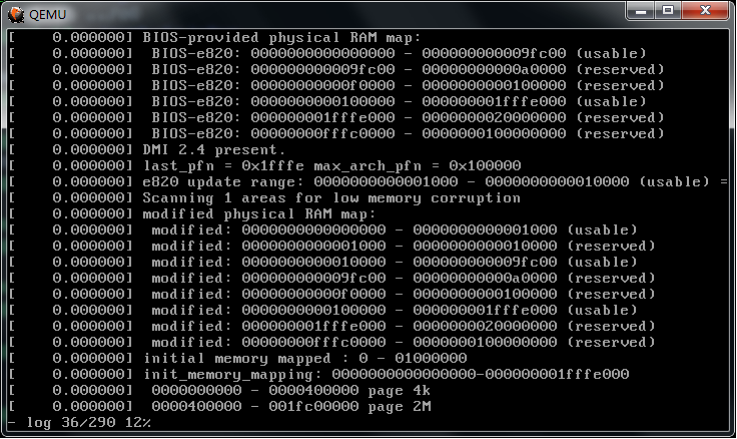
\includegraphics[scale=0.25]{images/e820}

\subsubsection{setup\_memory\_map}
在函数setup\_arch当中,setup\_memory\_map函数被调用,之后e820的memmap就做出了如图片当中的修改。它的内部调用了函数sanitize\_e820\_map,因为e820的某些memmap可能存在重叠,调用它的目的正是将这些重叠区域去掉。如果使用qemu来模拟机器是遇不到这种情况的。因此,我们直接避开他。


\subsection{通过early\_res分配内存}
e820仅仅保存了内存的布局信息,为了分配内存还需要做出进一步的努力以帮助系统记录那些内存被占用而那些内存仍可以被使用。在bootmem启动之前,承担这个责任的是early\_res,它与e820同样定义在文件arch/x86/kerenl/e820.c当中。结构体early\_res和它的一个全局数组early\_res便是记录内存分配信息的容器。
\begin{lstlisting}[language=C]
/*
 * Early reserved memory areas.
 */
#define MAX_EARLY_RES 20

struct early_res {
        u64 start, end;
        char name[16];
        char overlap_ok;
};
static struct early_res early_res[MAX_EARLY_RES] __initdata = {
        { 0, PAGE_SIZE, ``BIOS data page'' },     /* BIOS data page */
        {}
};
\end{lstlisting}
结构体当中overlap\_ok的意义比较复杂而且不算常用,暂且搁下后面介绍,结构器的其他字段意义比较明确也就不多说了。定义好了结构体之后,我们看看early\_res和e820如何配合分配内存。起到关键作用是函数find\_e820\_area和函数reserve\_early,其中函数find\_e820\_area的作用是寻找空闲区域而reserve\_early的作用是标记指定内存已经被分配。Linux当中包含很多这样的应用常见,例如下面的代码

\begin{lstlisting}[language=C]
// arch/x86/mm/init_32.c
void __init setup_bootmem_allocator(void) {
  bootmap_size = bootmem_bootmap_pages(max_low_pfn)<<PAGE_SHIFT;
  // find_e820_area从全局变量e820当中寻找一个能够容纳指定内存的段,且此段
  // 同时拥有足够的内存尚未被 reserve_early占用。
  // 而后使用reserve_early分配内存,实际上仅仅是在early_res数组当中增加一项
  // 告知内存已经被分配。
  bootmap = find_e820_area(0, max_pfn_mapped<<PAGE_SHIFT, bootmap_size,
                          PAGE_SIZE);
  reserve_early(bootmap, bootmap + bootmap_size, ``BOOTMAP'');
}
\end{lstlisting}
这段代码的作用是为bootmem的结构体分配空间。
\subsubsection{find\_e820\_area的实现}
\begin{algorithm}[H]
\SetAlgoLined
\BlankLine
\For{item in e820} {
  \If {item不是可分配内存或者空间不足} {
    continue;
  }
  \If {item当中未分配的内存已经不足} {
   continue;
  }
  返回内存地址
}
\BlankLine
返回空

\caption{find\_e820\_area}
\end{algorithm}

\subsection{与early\_res分配相关的函数}
\begin{itemize}
\item find\_overlapped\_early(u64 s, u64 e);
\item drop\_range(int i) 丢弃第i个slot
\item drop\_overlaps\_that\_are\_ok(u64 s, u64 e);
\item \_\_reserve\_early(u64 s, u64 e, char* name, int overlap)
\item reserve\_early\_overlap\_ok(u64 start, u64 end, char *name)
\end{itemize}

\subsection{overlap\_ok}

结构体early\_res的意义还是比较明确的,除了overlap\_ok,这个名字会让人误会以为它是“此区域可以覆盖更早的分配",但实际却不是这样,它的解释在函数reserve\_early\_overlap\_ok处。
\begin{lstlisting}[language=C]
/*
 * A few early reservtations come here.
 *
 * The 'overlap_ok' in the name of this routine does -not- mean it
 * is ok for these reservations to overlap an earlier reservation.
 * Rather it means that it is ok for subsequent reservations to
 * overlap this one.
 *
 * Use this entry point to reserve early ranges when you are doing
 * so out of "Paranoia", reserving perhaps more memory than you need,
 * just in case, and don't mind a subsequent overlapping reservation
 * that is known to be needed.
 *
 * The drop_overlaps_that_are_ok() call here isn't really needed.
 * It would be needed if we had two colliding 'overlap_ok'
 * reservations, so that the second such would not panic on the
 * overlap with the first.  We don't have any such as of this
 * writing, but might as well tolerate such if it happens in
 * the future.
 */
\end{lstlisting}

它的意思实际上是分配的内存可以在之后的分配时被overlap,即被使用。

\subsection{early\_res的应用场景}


\section{bootmem}
\subsection{为何需要bootmem}
bootmem的主要代码在mm/bootmem.c当中,从路径就可以看出bootmem已经是一个架构无关的内存管理框架了。

\subsection{bootmem框架}
bootmem使用bootmem\_data\_t来保存分配的内存,而且为了不再受到静态数组大小的限制,bootmem使用链表来记录分配的内存记录,这也是个巨大的飞跃。
\begin{lstlisting}[language=C]
// 文件 include/linux/bootmem.h
/*
 * node_bootmem_map is a map pointer - the bits represent all physical
 * memory pages (including holes) on the node.
 */
typedef struct bootmem_data {
  /* 当前节点负责管理的开始页帧及结束页帧 [node_min_pfn, node_low_pfn)
  unsigned long node_min_pfn;
  unsigned long node_low_pfn;
  
  /* 页帧使用情况的 bitmap */
  void *node_bootmem_map;
  unsigned long last_end_off;
  unsigned long hint_idx;
 
  /* 指向下一个节点 */
  struct list_head list;
} bootmem_data_t;

// 全局变量定义在 mm/bootmem.c 当中
bootmem_data_t bootmem_node_data[MAX_NUMNODES];
\end{lstlisting}

\subsubsection{bootmem初始化}
bootmem的初始化工作由init\_bootmem来完成,它通过调用init\_bootmem\_core来完成具体工作。
\begin{lstlisting}[language=C]
/**
 * init_bootmem - register boot memory
 * @start: pfn where the bitmap is to be placed
 * @pages: number of available physical pages
 *
 * Returns the number of bytes needed to hold the bitmap.
 */
unsigned long __init init_bootmem(unsigned long start, unsigned long pages)
{
  max_low_pfn = pages;
  min_low_pfn = start;

  /* NODE_DATA 访问的是 bootmem_node_data
   * 此处 bootmem 将由 start 开始的 pages 个页帧交给 bootmem 管理
   */
  return init_bootmem_core(NODE_DATA(0)->bdata, start, 0, pages);
}

static unsigned long __init init_bootmem_core(bootmem_data_t *bdata,
  unsigned long mapstart, unsigned long start, unsigned long end) {
  unsigned long mapsize;


  /* 此函数完成一些验证工作,并根据限制条件修改start和end的值 */
  mminit_validate_memmodel_limits(&start, &end);
  bdata->node_bootmem_map = phys_to_virt(PFN_PHYS(mapstart));
  bdata->node_min_pfn = start;
  bdata->node_low_pfn = end;

  /*
  * link_bootmem将bdata 放在合适的链表的位置上
  * 以保证链表是按照升序排列的
  */
  link_bootmem(bdata);

  /*
   * Initially all pages are reserved - setup_arch() has to
   * register free RAM areas explicitly.
   */
  mapsize = bootmap_bytes(end - start);
  memset(bdata->node_bootmem_map, 0xff, mapsize);

  return mapsize;
}

\end{lstlisting}

\subsection{分配内存}
分配内存的过程对于理解内存管理由为重要,bootmem提供了一组函数完成这些工作。首先来看页帧的分配和释放。
\subsubsection{page frame的分配和释放}
\begin{lstlisting}[language=C]
/* 此函数的功能是释放数据节点 bdata 的页帧
 * 范围是从 sidx 到 edix
 */
static void __init __free(bootmem_data_t *bdata,
                        unsigned long sidx, unsigned long eidx)
{
  unsigned long idx;
  if (bdata->hint_idx > sidx)
    bdata->hint_idx = sidx;

   /* 在 bitmap 上标记为可用 */
   for (idx = sidx; idx < eidx; idx++)
     if (!test_and_clear_bit(idx, bdata->node_bootmem_map))
       BUG();
}

/*
 * 分配从 sidx 到 edix 为止的页帧
 */
static int __init __reserve(bootmem_data_t *bdata, unsigned long sidx,
                        unsigned long eidx, int flags)
{
  unsigned long idx;
  int exclusive = flags & BOOTMEM_EXCLUSIVE;

  for (idx = sidx; idx < eidx; idx++)
    if (test_and_set_bit(idx, bdata->node_bootmem_map)) {
      if (exclusive) {
        __free(bdata, sidx, idx);
        return -EBUSY;
     }
  }
  return 0;
}

\end{lstlisting}
\subsubsection{bytes级别的分配与释放}
上面介绍了页帧的分配和释放,一般情况下,页帧最小也要4K,一般来说很少能一次用到这么多的内存,更多的情况还是以字节为单位分配的居多。
\begin{lstlisting}[language=C]
/**
 * __alloc_bootmem - allocate boot memory
 * @size: size of the request in bytes
 * @align: alignment of the region
 * @goal: preferred starting address of the region
 *
 * The goal is dropped if it can not be satisfied and the allocation will
 * fall back to memory below @goal.
 *
 * Allocation may happen on any node in the system.
 *
 * The function panics if the request can not be satisfied.
 */
void * __init __alloc_bootmem(unsigned long size, unsigned long align,
                              unsigned long goal)
{
  return ___alloc_bootmem(size, align, goal, 0);
}

static void * __init ___alloc_bootmem_nopanic(unsigned long size,
                                              unsigned long align,
                                              unsigned long goal,
                                              unsigned long limit)
{
  bootmem_data_t *bdata;
  void *region;

restart:
  region = alloc_arch_preferred_bootmem(NULL, size, align, goal, limit);
  if (region)
    return region;

  /* 对于 x86 来说, alloc_arch_preferred_bootmem 已经尝试了从
   * NODE_DATA(0) 处分配内存
   */
  list_for_each_entry(bdata, &bdata_list, list) {
    if (goal && bdata->node_low_pfn <= PFN_DOWN(goal))
      continue;
    if (limit && bdata->node_min_pfn >= PFN_DOWN(limit))
      break;

    region = alloc_bootmem_core(bdata, size, align, goal, limit);
    if (region)
      return region;
  }

  if (goal) {
    goal = 0;
    goto restart;
  }

  return NULL;
}

static void * __init alloc_arch_preferred_bootmem(bootmem_data_t *bdata,
                                                  unsigned long size,
                                                  unsigned long align,
                                                  unsigned long goal,
                                                  unsigned long limit) {
  if (WARN_ON_ONCE(slab_is_available()))
    return kzalloc(size, GFP_NOWAIT);

#ifdef CONFIG_HAVE_ARCH_BOOTMEM
  {
    bootmem_data_t *p_bdata;
    /* bootmem_arch_preferred_node 是一个宏,
     *  定义在 arch/x86/include/asm/mmzone_32.h 
     * 它返回 (NODE_DATA(0)->bdata) 
     */
    p_bdata = bootmem_arch_preferred_node(bdata, size, align,
                                          goal, limit);
    if (p_bdata)
      return alloc_bootmem_core(p_bdata, size, align,
                                goal, limit);
  }
#endif
  return NULL;
}


static void * __init alloc_bootmem_core(struct bootmem_data *bdata,
                                        unsigned long size, unsigned long align,
                                        unsigned long goal, unsigned long limit)
{
  unsigned long fallback = 0;
  unsigned long min, max, start, sidx, midx, step;

  if (!bdata->node_bootmem_map)
    return NULL;

  min = bdata->node_min_pfn;
  max = bdata->node_low_pfn;

  goal >>= PAGE_SHIFT;
  limit >>= PAGE_SHIFT;

  if (limit && max > limit)
    max = limit;
  if (max <= min)
    return NULL;

  /* 根据对其方式获取每次得到多少个页 */
  step = max(align >> PAGE_SHIFT, 1UL);

  if (goal && min < goal && goal < max)
    start = ALIGN(goal, step);
  else
    start = ALIGN(min, step);

  sidx = start - bdata->node_min_pfn;
  midx = max - bdata->node_min_pfn;

  if (bdata->hint_idx > sidx) {
    /*
     * Handle the valid case of sidx being zero and still
     * catch the fallback below.
     */
    fallback = sidx + 1;
    sidx = align_idx(bdata, bdata->hint_idx, step);
  }

  while (1) {
    int merge;
    void *region;
    unsigned long eidx, i, start_off, end_off;
 find_block:
    sidx = find_next_zero_bit(bdata->node_bootmem_map, midx, sidx);
    sidx = align_idx(bdata, sidx, step);
    eidx = sidx + PFN_UP(size);

    if (sidx >= midx || eidx > midx)
      break;

    for (i = sidx; i < eidx; i++)
      /* 测试接下来的几个 bit 是否处于可分配状态 */
      if (test_bit(i, bdata->node_bootmem_map)) {
        sidx = align_idx(bdata, i, step);
        if (sidx == i)
          sidx += step;
        goto find_block;
      }

    if (bdata->last_end_off & (PAGE_SIZE - 1) &&
        PFN_DOWN(bdata->last_end_off) + 1 == sidx)
      start_off = align_off(bdata, bdata->last_end_off, align);
    else
      start_off = PFN_PHYS(sidx);

    merge = PFN_DOWN(start_off) < sidx;
    end_off = start_off + size;

    bdata->last_end_off = end_off;
    bdata->hint_idx = PFN_UP(end_off);

    /* 分配内存,记录到 bitmap 上 */
    if (__reserve(bdata, PFN_DOWN(start_off) + merge,
                  PFN_UP(end_off), BOOTMEM_EXCLUSIVE))
      BUG();

    /* 将内存转化为虚拟内存 */
    region = phys_to_virt(PFN_PHYS(bdata->node_min_pfn) +
                          start_off);
    memset(region, 0, size);
    /*
     * The min_count is set to 0 so that bootmem allocated blocks
     * are never reported as leaks.
     */
    kmemleak_alloc(region, size, 0, 0);
    return region;
  }

  /* fallback 的作用 */
  if (fallback) {
    sidx = align_idx(bdata, fallback - 1, step);
    fallback = 0;
    goto find_block;
  }

  return NULL;
}

\end{lstlisting}

\subsection{early\_res到bootmem的转换}
在early\_res的工作完成以后,操作系统将内存管理的任务交给bootmem管理。转交过程中起到最大作用的是函数early\_res\_to\_bootmem,它将early\_res当中分配的内存转到bootmem的内存管理框架下。

\section{变量命名规则}
\begin{itemize}
\item pfn:  page frame num
\item va:   vitural address
\item pa:   physical address
\end{itemize}
\end{document}

\section{x86分页模式}

\subsection{反汇编}
在启用分页之后,反汇编将变得有些令人迷惑。在启动分页模式之前,调试总是针对物理地址的,这时候使用的指令是hbreak;启动分页模式之后,如果依然按照之前的方法进行,读者一定会发现与地址相关的值是转换为硬件地址之后的值,而非虚拟地址,这多少会令人疑惑分页机制到底启用没有。没关系,验证的方法总是有的,通过反汇编虚拟地址是一个不错的办法。

使用gdb对虚拟地址进行反汇编
\begin{lstlisting}
(gdb) disas 0xc0100000,+100
Dump of assembler code from 0xc0100000 to 0xc0100064:
   0xc0100000 <startup_32+0>:   cld
   0xc0100001 <startup_32+1>:   lgdtl  0x100294
   0xc0100008 <startup_32+8>:   mov    $0x10,%eax
   0xc010000d <startup_32+13>:  mov    %eax,%ds
   0xc010000f <startup_32+15>:  mov    %eax,%es
   0xc0100011 <startup_32+17>:  mov    %eax,%fs
   0xc0100013 <startup_32+19>:  mov    %eax,%gs
   0xc0100015 <startup_32+21>:  mov    %eax,%ss
   0xc0100017 <startup_32+23>:  mov    $0x105000,%edi
   0xc010001c <startup_32+28>:  mov    $0x101000,%edx
   0xc0100021 <startup_32+33>:  mov    $0x7,%eax
   0xc0100026 <startup_32+38>:  lea    0x7(%edi),%ecx
   0xc0100029 <startup_32+41>:  mov    %ecx,(%edx)
   0xc010002b <startup_32+43>:  mov    %ecx,0xc00(%edx)
   0xc0100031 <startup_32+49>:  add    $0x4,%edx
   0xc0100034 <startup_32+52>:  mov    $0x400,%ecx
   0xc0100039 <startup_32+57>:  stos   %eax,%es:(%edi)
   0xc010003a <startup_32+58>:  add    $0x1000,%eax
   0xc010003f <startup_32+63>:  loop   0xc0100039 <startup_32+57>
   0xc0100041 <startup_32+65>:  lea    0x20007(%edi),%ebp
   0xc0100047 <startup_32+71>:  cmp    %ebp,%eax
   0xc0100049 <startup_32+73>:  jb     0xc0100026 <startup_32+38>
   0xc010004b <startup_32+75>:  mov    %edi,0x1002a0
   0xc0100051 <startup_32+81>:  mov    $0x101000,%eax
   0xc0100056 <startup_32+86>:  mov    %eax,%cr3
   0xc0100059 <startup_32+89>:  mov    %cr0,%eax
   0xc010005c <startup_32+92>:  or     $0x80000000,%eax
   0xc0100061 <startup_32+97>:  mov    %eax,%cr0
End of assembler dump.
\end{lstlisting}


使用gdb对物理地址进行反汇编
\begin{lstlisting}
(gdb) disas 0x100000,+100
Dump of assembler code from 0x100000 to 0x100064:
=> 0x00100000:  cld
   0x00100001:  lgdtl  0x1000fc
   0x00100008:  mov    $0x18,%eax
   0x0010000d:  mov    %eax,%ds
   0x0010000f:  mov    %eax,%es
   0x00100011:  mov    %eax,%fs
   0x00100013:  mov    %eax,%gs
   0x00100015:  mov    %eax,%ss
   0x00100017:  mov    $0x104000,%edi
   0x0010001c:  mov    $0x101000,%edx
   0x00100021:  mov    $0x7,%eax
   0x00100026:  lea    0x7(%edi),%ecx
   0x00100029:  mov    %ecx,(%edx)
   0x0010002b:  mov    %ecx,0xc00(%edx)
   0x00100031:  add    $0x4,%edx
   0x00100034:  mov    $0x400,%ecx
   0x00100039:  stos   %eax,%es:(%edi)
   0x0010003a:  add    $0x1000,%eax
   0x0010003f:  loop   0x100039
   0x00100041:  lea    0x20007(%edi),%ebp
   0x00100047:  cmp    %ebp,%eax
   0x00100049:  jb     0x100026
   0x0010004b:  mov    %edi,0x100108
   0x00100051:  mov    $0x101000,%eax
   0x00100056:  mov    %eax,%cr3
   0x00100059:  mov    %cr0,%eax
   0x0010005c:  or     $0x80000000,%eax
   0x00100061:  mov    %eax,%cr0
End of assembler dump.
\end{lstlisting}

对比结果可以很明显的发现其中的差别,针对虚拟地址的反汇编的地址值基本都是0xC001****格式的,因为gdb做了一些转换工作,如果不知道这种转换的存在,相信调试者一定会很迷惑。因为作者就曾经很迷惑:到底分页机制启用了没有。作者还尝试使用objdump的反汇编结果与物理地址反汇编结果向对比,差别于此类似,当却让作者开始怀疑虚拟机的正确性。还有“交叉验证”的方式总是能够帮助更进一步的理解问题。

\part{基本设备驱动程序}
\chapter{驱动程序框架}

\chapter{键盘}

\chapter{控制台及终端}

\section{printk}
\subsection{early-printk}
early-printk是初始化时期的printk的实现。Linux为了提供类似功能的通用初始化架构,利用了一些技巧,这些技巧很多其他模块都用到了。


setup\_early\_printk是初始化early\_printk的函数,通过宏early\_param将初始化printk的函数setup\_early\_printk的存放在obs\_kernel\_param数组当中。

\begin{lstlisting}[language=c]

// 文件 arch/x86/kernel/early_printk.c
early_param("earlyprintk", setup_early_printk);


// 文件 include/kernel/init.h
/*
 * Only for really core code.  See moduleparam.h for the normal way.
 *
 * Force the alignment so the compiler doesn't space elements of the
 * obs_kernel_param ``array'' too far apart in .init.setup.
 */
#define __setup_param(str, unique_id, fn, early)                        \
        static const char __setup_str_##unique_id[] __initconst \
                __aligned(1) = str; \
        static struct obs_kernel_param __setup_##unique_id      \
                __used __section(.init.setup)                   \
                __attribute__((aligned((sizeof(long)))))        \
                = { __setup_str_##unique_id, fn, early }

#define __setup(str, fn)                                        \
        __setup_param(str, fn, fn, 0)

/* NOTE: fn is as per module_param, not __setup!  Emits warning if fn
 * returns non-zero. */
#define early_param(str, fn)                                    \
        __setup_param(str, fn, fn, 1)

\end{lstlisting}
从上面的代码可以看到,\_\_setup\_param的数据以struct obs\_kernel\_param的结构存放并置与.init.setup段当中,这个段专门用来存储初始化阶段的数据,且全部以结构体obs\_kernel\_param的结构存储。通过段指令,即使early\_param宏存放与不同的文件当中,但数据仍然是连续存储的,它看起来就像一个数组。

连续存放的文件解决了,接下来探究一下Linux是如何访问这些数据的,毕竟每次修改代码,这些数据的位置都会改变,因此它们的地址是不固定的,也就是说不能通过制定地址常量的方式来访问。Linux通过定义在lds当中的全局变量来定位.init.setup的起始及结束地址,这种技巧也是Linux非常常用的技巧之一。
\begin{lstlisting}
__setup_start = .;
.init.setup : { *(.init.setup) }
__setup_end = .;
\end{lstlisting}

而后在init/main.c当中就可以通过两个外部变量来遍历这个数组了。
\begin{lstlisting}[language=c]

extern struct obs_kernel_param __setup_start[], __setup_end[];
static int do_early_param(char* param, char* val) {
  for (p = __setup_start; p < __setup_end; p++) {
    /* code */
  }
}
\end{lstlisting}

\documentclass[b5paper,9pt,twoside,openany]{article}
\usepackage{fontspec,xunicode,xltxtra}
\usepackage{listings}
\usepackage{color}
\usepackage{paralist}
\usepackage{qtree}
\usepackage{dirtree}
\usepackage{pstricks,pst-node}
\usepackage{tabularx}
\usepackage[a5paper]{geometry}
\usepackage[colorlinks=true,linkcolor=blue]{hyperref}


\XeTeXlinebreaklocale ``zh''
\XeTeXlinebreakskip = 0pt plus 1pt minus 0.1pt
\newfontfamily\song{SimSun}
\newfontfamily\hei{SimHei}
%\newfontfamily\kai{KaiTi}
%\newfontfamily\fsong{FangSong}
%\newfontfamily\nsong{NSimSun}
\newfontfamily\mshei{Microsoft YaHei}
\setmainfont{SimSun}


\begin{document}
\includegraphics{fig.1}
\end{document}

\chapter{ext2文件系统}

\chapter{proc文件系统}


\part{兼容Linux}
\chapter{系统调用}

在文件系统ready以后,我们可以开始运行文件系统上的程序了。
加载一个程序可能很简单,但真的运行它就没有那么容易了。
首先要注意的这个程序一定是在其他形同上编译链接的,运行简单的指令当然没有问题。
但时当程序需要I/O,网络,文件等等复杂操作该怎么办呢?
从本质上讲,这些复杂的操作都是“系统调用”。
只要我们的系统调用与Linux保持兼容,那么Linux可以运行的程序,理论上就可以在我们的系统上运行。

为了向伟大的“Hello, World”致敬,我们就从它开始,让他成为第一个可以运行在我们系统之上的程序。
\section{Hello, World}

\chapter{动态库的加载}
从第一章开始,我们就与ELF文件打交道了。
Linux的动态库也是ELF文件,需要动态链接的应用程序简单来说就是把动态连接库的ELF文件加载到用户空间罢了。
基本原理非常简单,不过细节还是要关注的。


\part{Linux高级特性}
\chapter{多线程}

\chapter{Linux信号处理}

\chapter{互斥与同步}
\section{原子操作}
对于同步问题来说,其中最简单的操作就是“原子操作”。原子操作的概念

\chapter{用户模式Linux}

\chapter{虚拟化技术}


\part{x86高级特性}
\chapter{x86 APIC}
本章介绍x86下CPU的APIC(高级可编程中断控制器),”高级“这两个字可以看作是跟之前PIC相对应的。
APIC也是支持SMP的基础,下一章回介绍SMP,那将是非常复杂的部分。

\chapter{对称多核结构}


\part{附录}
\appendix
\chapter{GNU Toolchain1}


\section{GNU AS简介}
\section{GNU AS}
\section{GAS常用技巧}
在初始化阶段,Linux用到一些高阶技巧,这些技巧结合了伪指令,代码和数据及连接器,
需要返回推敲Linux的源代码才能明白他的用意。
\subsection{数组初始化}
这里以interrrupts的idt初始化为例,介绍GNU AS通过段切换来达到初始化数组的目的。

首先需要熟悉的是 .section 指令,这个指令通知汇编器:从现在开始之后的代码属于指定段。
\section{GNU C嵌入汇编}

\chapter{Makefile}
Makefile是一款非常著名的项目管理软件,虽然说它不好的人很多但用它的人更多。你能角的出名字的大公司基本都用它。Linux也是使用Makefile来管理真个项目的。这一张将介绍Linux当中的Makefile使用。Linux的Makefile涉及到非常多的技巧,我们以下三个方面来介绍:首先是Makefile基本语法;第二部分介绍我们的Makefile,这是一个与Linux makefile基本类似,但经过极大简化的Build系统,在了解了它以后,了解Linux的kbuild系统就没有什么问题了。最后我们介绍Linux的Makefile,到了这里只要介绍几下Makefile的基本机制,相信大家自己都能想清楚了。



 \section{Makefile基础}
Makefile最基本的单位是目标,最基本的关系是依赖。一个项目可以有多个目标组成,其中每一个目标又依赖于很多个.o文件。每一个.o文件依赖于.c文件。根据这些依赖关系可以支撑一个森林(多棵树)。如果希望生成其中任何一个目标只要从树顶开始进行后序编译即可。
\subsection{Makefile基础}
接下来我们从一个简单的设计多文件的程序来更具体的理解Makefile的工作方式。
\begin{lstlisting}[language=make]
CFLAGS = -c
default: hello
hello : hello.o lib.o
   ld  ${LDFLAGS} hello.o lib.o -o hello

hello.o: hello.c
   gcc ${CFLAGS} hello.c -o hello.o

lib.o: lib.c
   gcc ${CFLAGS} lib.c -o lib.o
\end{lstlisting}

正如之前提到的,这段代码可以用森林表示,但这森林很小仅仅有一个小树:


\qtreecentertrue 
\Tree [.default [.hello [.hello.o \textit{gcc hello.c -o hello.o} ] 
                        [.lib.o \textit{gcc lib.c -o lib.o} ] ] ]


Makefile的内部实现基本上也是以树为组织形式,而后通过后续遍历。
按照先生成依赖项而后生成自身的顺序完成整个工程的构建。


此外,make还有一个很好的特性:它会监控每一个依赖项及target的变化。如果其中任何一个改变,那么所有依赖于它的项(包括直接依赖及间接依赖)都会被重新生成。这个特性很好,尤其是当项目设计非常多的文件的时候,如果一个文件变化导致整个项目重新build那就太耗时了。
\subsection{伪目标}
实际上Makefile会将所有的target及依赖项当作文件,如果目标不是一个文件会怎么样呢?make会把它当作文件并理所当然的认为它被存在是因为没有被生成,因此这个目标总是被执行。最常见的伪目标是clean。例如给上面的Makefile加上clean:
\begin{lstlisting}[language=make]
CFLAGS = -c
default: hello
hello : hello.o lib.o
   ld  ${LDFLAGS} hello.o lib.o -o hello

hello.o: hello.c
   gcc ${CFLAGS} hello.c -o hello.o

lib.o: lib.c
   gcc ${CFLAGS} lib.c -o lib.o

clean:
    rm -f *.o
    rm -f hello
.PHONY: clean
\end{lstlisting}
每当我们运行make clean的时候,两条rm命令都会执行,因为clean是不存的。make提供了一个特殊的指令叫做.PHONY,它可以用于表示伪目标,但一般不会这么做。

Makefile的内部实现基本上也是以树为组织形式,而后通过后续遍历。
按照先生成依赖项而后生成自身的顺序完成整个工程的构建。

此外,make还有一个很好的特性:它会监控每一个依赖项及target的变化。如果其中任何一个改变,那么所有依赖于它的项(包括直接依赖及间接依赖)都会被重新生成。这个特性很好,尤其是当项目设计非常多的文件的时候,如果一个文件变化导致整个项目重新build那就太耗时了。
\subsection{Makefile变量}
和众多脚本语言一样,Makefile怎么可能没有变量呢。上面的例子就有两个变量\$\{LDFLAGS\}和变量\$\{CFLAGS\}。
变量定义的格式比较直接一个赋值运算符就可以搞定了。

GNU Make当中包含两种复制运算符“=”和“:=”。这两个运算符还是有一些差异的。赋值符号“:=“会立刻计算右边的字符串并赋值给变量。而运算符“=”则会仅仅保存表达式,在用到变量的一刻,make程序会计算(evaluate)它的值并加入到运算当中。我们通过一个例子来了解一下他们的不同。这非常重要,因为Linux的Makefile当中这种技巧用了很多。

\subsection{Makefile函数调用}
如果单单认为Makefile就是这么简单的话,恐怕会让大家失望。
如果只是这么简单,我们也就不用单独开辟一章来介绍Linux Kernel的Makefile了。
实际上Makefile包含非常多的强大功能,对于很多支持多平台的软件来说,这些功能都是不可或缺的。
接下来我们介绍函数调用。
\subsection{Makefile流程控制}
大部分介绍编程语言书籍来都倾向于将流程控制放在函数之前,这这里我们却不得不成为一个例外。
原因很简单,Makefile的流程控制是基于函数调用的,它并没有关键字if,或是关键字for,
它拥有的是两个函数if和foreach。
这两个函数是Makefile流程控制的基础。
\subsubsection{if}
\subsubsection{foreach}
还是通过例子来学习它吧
\begin{lstlisting}[language=make]
srcs := a.c b.c c.c
files := $(foreach,n,${srcs},$(shell gcc -c ${n} -o ${n}.o))
\end{lstlisting}
函数for有4个参数
\begin{itemize}
\item n 用于枚举,代表一次迭代从参数srcs当中取出的值
\item \$\{srcs\} 用于枚举的对象
\item 循环体 \$(shell gcc \-c \$\{n\} \-o \$\{n\}.o) 
\end{itemize}

 \section{简化kbuild}
本着山寨的精神,Linux的Makefile也是需要改造一把的。不是为了让他变得更好,只是为了让它变得更简单,更容易理解。下面的章节将介绍kbuild系统的如何实现,当然那些高级配置部分的实现被省去了,作为一个仅仅支持x86的简陋操作系统,实在不需要配置啊。

\subsection{生成built-in}
kbuild通过脚本的方式将所有的obj-y文件通过\${LD} \-r当方式连接成为built\-in.o文件。
之后built\-in.o会被链接成为vmlinux文件。
有一点需要注意的时,obj\-y当中的文件是可以重复出现的,但仅仅第一次出现是有效的。
不过前面提到过这些文件对应的源代码文件有是汇编程序也有可能是C程序,它们是如何确定源文件路径及名称的。又是如何确定编译选项的?
下面的代码会给你答案。

\section{稍许改造}
\subsection{sysmap}
为了调试方便Linux在生成玩vmlinux之后,还通过nm命令生成了一张记录所有符号地址的表保存在文件当中。我们不打算这么做,毕竟去查表也是挺复杂的一件事情,为了方便起见我们还是使用gdb调试。因为我们在链接阶段生成两个版本的vmlinux。一个包含调试信息,它仅仅用来帮助调试器识别符号及变量。另外一个文件不太调试信息它将被写入到磁盘当中作为操作系统运行。无论生成那种文件,在编译阶段都通过选项-g使其包含调试信息。在链接不包含调试信息的版本是用 ld -s(或者--strip-all) 生成即可。--strip-all选项会取出所有符号相关的信息。
\subsection{输出路径}
很多年以前开始使用VC,它倾向于将生成的代码放在一个名为debug(或者release)的目录下以便于管理。
后来Visual Studio用的多了,发现这并不是一个很好的特性。
随着Solution的复杂度提升,更多的项目加入到了其中,每一个项目都有自己一个debug和release目录。
当我看到chromium的项目组织的时候,我非常的钦佩,我认为那是更好的输出文件组织形式。

\section{Linux构建系统介绍}
\subsection{kbuild Makefile基本语法}
Linux Kernel的Makefile通过变量来记录那些文件需要build以及文件作为什么的组成部分。Linux Kerne的Makefiles在官方文档上被曾作kbuild Makefiles,我们也称他为kbuild Makefiles。
大致上,内核的不表包括两种built-in以及module。
build-in代表的是整个内核,如果文件需要编译进到vmlinux这个ELF文件,那么通常它会在Makefile当中写作
 \begin{lstlisting}[language=make]
  obj-y += foo.o
 \end{lstlisting}
否则话可能写作
 \begin{lstlisting}[language=make]
  obj-m += foo.o
 \end{lstlisting}
当然还有一种情况就是根据用户的配置进行生成
 \begin{lstlisting}[language=make]
  obj-${CONFIG_FOO} += foo.o
 \end{lstlisting}
如果CONFIG\_FOO被配置成y, 那么他就被直接编译到built\-in当中,如果配置为m,则别生成为可加载的内容。除了obj-m和obj-y两个目标之外,还有目标lib-y,这个目标下的所有文件会被用来生成静态库lib.a。在最终的链接阶段它会被链接进vmlinux。
此外lib.a还会被发布供更多的应用程序使用。

\subsubsection{编译选项}
编译选项的管理使用与.o文件类似的管理方式。


此外KBUILD Makefile还提供了仅仅针对文件的编译方法。
\begin{lstlisting}[language=make]
 CFLAGS_aha152x.o = -DAHA152X_STAT -DAUTOCONF
\end{lstlisting}
这条CFLAGS仅仅用于当前subdir下的文件aha152x.o的生成。

\subsection{kbuild Commands}
kbuild系统中提供了很有常用的宏,链接它们对于阅读Linux Makefile非常有帮助。
\subsubsection{if\_changed}
可能读者会非常疑惑,前面提到,按道理Makefile会自己监控依赖项。如果依赖项变化了,Makefile会自己发现并重新生成直接依赖或者间接依赖次项的内容。那为什么还需要if\_chaneged这种功能呢?由GNU make自己来作者事情不是更好吗。
这是由于Linux的Makefile并没有按照最经典的依赖方式组织代码,这就造成了make无法监控更新,不得已需要有一个if\_changed这样的函数。
if\_changed有一个隐含约束,他检查的内容必须保存在变量\$\{targets\}当中。
\begin{lstlisting}[language=make]
 target: source(s) FORCE
     $(call if_changed,ld/objcopy/gzip)
\end{lstlisting}

Linux支持多种架构同时也支持多种编译器,但不同的编译器很多选项是不一样的,某些不同的编译器支持也不同。kbuild提供了一组函数用于判断当前使用的编译器是否支持指定选项。
这些函数包括cc\-option、cc\-option\-yn、cc\-option\-align、cc\-version等等。
在很多Makefile当中都可以找到使用它们的例子,如arch/i386/Makefile。
\begin{lstlisting}[language=make]
cflags-y += $(call cc-option,-march=pentium-mmx,-march=i586)
\end{lstlisting}
上面的代码会判断编译器是否支持“-march=pentium-mmx“,如果支持则使用。如果不支持就用“-march=i586”选项代替。

后面我们会尝试实现一个类似的Build系统,但由于我们只用GCC,这些函数我们就不用啦。为了方便读者自己阅读Linux的代码,我们在这里还是要顺便说明一下。


它们的实现在根目录的Makefile当中,基本都是通过shell命令完成的,如cc-option的实现如下。
\begin{lstlisting}[language=make]
cc-option = $(shell if $(CC) $(CFLAGS) $(1) \
               -S -o /dev/null -xc /dev/null \
               > /dev/null 2>&1; then \
               echo ``$(1)''; else echo ``$(2)''; fi ;)

\end{lstlisting}
\subsection{一些技巧}
上面介绍的是kbuild Makefile的整体,除了这些之外,它还用到了很多有趣的技巧。
\subsubsection{verbose}
verbose这个词用过linux的人一定非常熟,基本上所有的shell命令都有一个-v选项,它会把很多信息打出来。kbuild Makefile也提供了这样的功能,它的实现非常简单,但却值得看一下。

首先需要大家明白的一点是@, 它是常用的shell技巧,在make执行的时候如果不希望shell显示当前正在运行的命令就在前面加上@。例如
\begin{lstlisting}[language=make]
@echo "abc"
\end{lstlisting}
如果加上@, 他的输出就是
\begin{lstlisting}[language=bash]
"abc"
\end{lstlisting}
如果不加上@, 那么他的输出就是
\begin{lstlisting}[language=bash]
echo "abc"
"abc"
\end{lstlisting}

在顶层Makefile当中,你会发现下面一段代码
\begin{lstlisting}[language=make]
ifeq ($(KBUILD_VERBOSE),1)
  quiet =
  Q =
else
  quiet=quiet_
  Q = @
endif
\end{lstlisting}
在其他地方,如果Makefile用到了shell命令一定会写成

\begin{lstlisting}[language=make]
%.s: %.c scripts FORCE
    $(Q)$(MAKE) $(build)=$(@D) \$@
\end{lstlisting}


 \section{kbuild核心流程}
当用户在linux源代码目录下执行make的时候,构建系统就开始运作了。最开始执行的就是源代码根目录下的Makefile,linux的文档管它叫'top level Makefile'。
简单的说它包括如下共呢
\begin{compactenum}
\item 配置内核并产生.config文件
\item 生成include/linux/version.h文件
\item 根据目标arch的类型建立include/asm软链接
\item 更新所有的依赖
\item 递归的便利所有在init-*, core* drivers-* net-* libs*并build所有目标
\item 将生成的文件链接成vmlinux并存放在源代码根目录下
\item 最后准备用于安装的文件
\end{compactenum}

\subsection{变量初始化}
\subsubsection{LDFLAGS}
它是通用链接选项,所有的ld命令都会是用它
\subsubsection{LDFLAGS\_MODULE}
此选项用于生成可加载模块.ko的ld命令
\subsubsection{LDFLAGS\_vmlinux}
顾名思义,它是用于链接vmlinux的选项
\subsubsection{OBJCOPYFLAGS}
某些链接器不支持binary格式,此时可以通过objcopy命令来实现。例如
\begin{lstlisting}[language=bash]
OBJCOPYFLAGS := -O binary
# arch/i386/boot/Makefile
$(obj)/image: vmlinux FORCE
    $(call if_changed,objcopy)
\end{lstlisting}
\subsubsection{AFLAGS}
汇编程序的通用选项
\subsubsection{CFLAGS}
通用的C语言编译选项
\subsubsection{CFLAGS\_KERNEL}
生成内核的通用编译选项
\subsubsection{CFLAGS\_MODULE}
生成可加载模块的编译选项
\subsection{递归编译所有subdir}
真正的构建开始了,top level Makefile会按照一定次序递归访问subdir下的Makefile。这些子目录通过以下几个变量定义:
head-y、init-y、core-y、libs-y、drivers-y、net-y
\begin{compactenum}
\item head-y: 所有需要首先放到vmlinux的目标
\item libs-y: 所有用来生成lib.a的目录
\end{compactenum}
这些变量的定义分成两个部分,一部分在top level Makefile, 它定义了所有与平台架构无关的目录。另外一部分与平台相关的则定义在arch/\$\{ARCH\}/Makefile当中。
\begin{lstlisting}[language=make]
core-y += arch/i386/kernel/
libs-y += arch/i386/lib
drivers-$(CONFIG_OPROFILE)  += arch/sparc64/oprofile/
\end{lstlisting}

\subsection{kbuild Commands}
kbuild系统中提供了很有常用的宏,链接它们对于阅读Linux Makefile非常有帮助。
\subsubsection{if\_changed}
可能读者会非常疑惑,前面提到,按道理Makefile会自己监控依赖项。如果依赖项变化了,Makefile会自己发现并重新生成直接依赖或者间接依赖次项的内容。那为什么还需要if\_chaneged这种功能呢?由GNU make自己来作者事情不是更好吗。
这是由于Linux的Makefile并没有按照最经典的依赖方式组织代码,这就造成了make无法监控更新,不得已需要有一个if\_changed这样的函数。
if\_changed有一个隐含约束,他检查的内容必须保存在变量\$\{targets\}当中。
\begin{lstlisting}[language=make]
 target: source(s) FORCE
     $(call if_changed,ld/objcopy/gzip)
\end{lstlisting}

Linux支持多种架构同时也支持多种编译器,但不同的编译器很多选项是不一样的,某些不同的编译器支持也不同。kbuild提供了一组函数用于判断当前使用的编译器是否支持指定选项。
这些函数包括cc\-option、cc\-option\-yn、cc\-option\-align、cc\-version等等。
在很多Makefile当中都可以找到使用它们的例子,如arch/i386/Makefile。
\begin{lstlisting}[language=make]
cflags-y += $(call cc-option,-march=pentium-mmx,-march=i586)
\end{lstlisting}
上面的代码会判断编译器是否支持“-march=pentium-mmx“,如果支持则使用。如果不支持就用“-march=i586”选项代替。

后面我们会尝试实现一个类似的Build系统,但由于我们只用GCC,这些函数我们就不用啦。为了方便读者自己阅读Linux的代码,我们在这里还是要顺便说明一下。


它们的实现在根目录的Makefile当中,基本都是通过shell命令完成的,如cc-option的实现如下。
\begin{lstlisting}[language=make]
cc-option = $(shell if $(CC) $(CFLAGS) $(1) \
               -S -o /dev/null -xc /dev/null \
               > /dev/null 2>&1; then \
               echo ``$(1)''; else echo ``$(2)''; fi ;)

\end{lstlisting}

\section{Linux目录结构}
\dirtree{%
.1 rlinux.
.2 arch.
.3 i386.
.3 mm.
.3 kernel.
.3 mach-default.
.3 boot.
.2 drivers.
.2 fs.
.2 include.
.3 asm.
.3 asm-i386.
.3 linux.
.2 init.
.2 kernel.
.3 timers.
.2 lib.
.2 mm.
.2 scripts.
}

\chapter{调试技巧}
\section{使用gdb调试}
\subsection{gdb常用命令}
\subsubsection{查看内存}
\subsection{gdb基本原理}
\subsection{调试信息}

\section{使用bochs内置调试器}
bochs提供了一个内置调试题,只需要在配置文件当中添加如下一行便可以启动调试器了。带有调试器的bochs一开始运行便会自动定下,而后等待用户命令。
既然有了功能强大且通用的调试器gdb,为什么还需要bochs的内置调试器呢?它确实有着不可替代的作用,尤其是在刚开始入手的时候,内置调试的功能是gdb无法替代的。1
\subsection{查看内存}
\subsection{查看gdt}
\subsection{查看堆栈}
\subsection{日志}

\chapter{使用grub引导}
分析Linux代码是必不可少的,本章将介绍如何在磁盘镜像上安装grub并使用grub引导Linux。
\section{安装GRUB2}
\subsection{创建磁盘镜像}
创建磁盘的方法很多,本质上只是创建一个指定大小的内容全部为0的文件。这里采用bximage创建磁盘,它会顺便计算出磁盘的磁道,扇区数等信息,在创建分区的时候这些信息都是必要的。

\begin{lstlisting}[language=bash]
# 创建一个500M的磁盘
 bximage
 Do you want to create a floppy disk image or a hard disk image?
 Please type hd or fd. [hd] 

 What kind of image should I create?
 Please type flat, sparse or growing. [flat]

 Enter the hard disk size in megabytes, between 1 and 129023
 [10] 500

 I will create a 'flat' hard disk image with
  cyl=1015
  heads=16
  sectors per track=63
  total sectors=1023120
  total size=499.57 megabytes
\end{lstlisting}


在完成磁盘的创建以后,还需要对磁盘创建分区并格式化。Linux有一个非常方便的工具mtools可以完成功能,它提供了一组命令不需要将磁盘镜像映射成设备就可以对其操作。默认情况下linux是包含这个工具包的,可以通过命令sudo apt-get install mtools来安装。
\begin{lstlisting}[language=bash]
# mpartition -I C:
$ mpartition -cpv -t 1015 -h 16 -s 63 -b 63 C:
$ mformat C:
\end{lstlisting}

\subsection{加载磁盘}
在完成磁盘的创建以后,需要对磁盘镜像以块设备的方式进行操作。
\begin{lstlisting}[language=bash]
$ sudo losetup /dev/loop0 c.img
$ ls -l /dev/loop0
brw-rw---- 1 root disk 7, 0 Feb  4 14:56 /dev/loop0 # 7, 0 是主,次设备号
# 为磁盘的分区建立设备映射
$ sudo kpartx -v -a /dev/loop0
# 将分区映射到设备 /dev/loop1上
$ sudo losetup /dev/loop1 /dev/mapper/loop0p1
# 格式化磁盘
\end{lstlisting}

\subsection{安装grub2}

\begin{lstlisting}[language=bash]
$ sudo grub-install --no-floppy \
       --root-directory=/mnt \
       --modules=''fat ext2 part_msdos''  /dev/loop0
\end{lstlisting}

将c.img作为启动盘启动qemu,此时已经可以看到GRUB2的提示符号了
\begin{lstlisting}
qemu-system-i386 -hda c.img
\end{lstlisting}

\subsection{关闭磁盘映射}
\begin{lstlisting}[language=bash]
# 关闭映射设备
$ sudo kpartx -d /dev/loop1
$ sudo losetup -d /dev/loop1
$ sudo losetup -d /dev/loop0
\end{lstlisting}
\section{安装Linux}
\subsection{安装内核文件}
将编译成功的Linux拷贝到文件镜像下,通常这个文件处于
arch/x86/boot/vmlinux
\begin{lstlisting}[language=bash]
mcopy arch/x86/boot/vmlinux c:
\end{lstlisting}
\subsection{配置grub}
打开一个文件并输入
\begin{lstlisting}[language=bash]

menuentry "My Linux Kernel" {
  set root='(hd0,msdos1)'
  linux /linux/vmlinuz ro
  initrd /linux/initrd.img
  insmod gzio
  insmod part_msdos
  insmod ext2
}
mcopy grub.cfg c:/boot/
\end{lstlisting}


\subsection{启动}
启动qemu,在启动grub cli之后输入
\begin{lstlisting}[language=bash]
grub> configfile /boot/grub.cfg
grub> boot
\end{lstlisting}
此时应该可以在屏幕当中看到内核启动了。
\section{安装GRUB2}

\chapter{交叉编译}
仅仅阅读内核是远远不够的,如果能够动态跟踪内核的执行路径,对于理解内核有莫大的帮助。鉴于我们的内核主要面向i386架构,而时下流行的机器及操作系统全部是64位系统,读者是没有办法直接编译32位内核的,必须使用一些功能才能做到。在这方面的投资绝对是值得的,随着对内核理解的加深,如果希望在手机等移动设备平台上调试内核,这些工具都是要熟悉的。

\section{crosstool-ng}
crosstool-ng也是GNU的开源项目,它能够自动下载,编译并生成cross compiler所需要的所有工具,库及操作系统。值得一提的是,某些代码并不能直接编译,需要打些patch,这些工作crosstool-ng都能够自动完成。

\begin{lstlisting}
ct-ng menuconfig
ct-ng build.8
\end{lstlisting}

\section{依赖项}
在开始交叉编译之前,需要安装一系列的编译工具,它们包括



这些工具很容易获取,无论是在linux平台还是在cgywin上,它们都是很基础的包。

\section{常见错误}
编译工具如果在cgywin平台上编译可能会出现大小写的问题,默认情况下windows的文件名不是大小写敏感的,而某些开源软件的代码文件必须要保证这点,否则将会出现文件被覆盖等错误。好在微软并没有堵死“大小写敏感”,用户可以通过注册表来修改“大小写敏感”选项。具体的注册表键值设置如下:
\begin{lstlisting}
 Windows Registry Editor Version 5.00

 [HKEY_LOCAL_MACHINE\SYSTEM\CurrentControlSet\Control\Session Manager\kernel]
``obcaseinsensitive''=dword:00000000
\end{lstlisting}









\chapter{Linux内核名词表}

\chapter{参考文献}

\backmatter
\end{document}
